% !TEX root = ../Diplombericht.tex
\subsection{Physischer Aufbau}

\subsubsection{Komponenten Platzierung}
Der Cluster ist in einem Gestell, welches 4 Ebenen hat, implementiert. Die Ebenen sind wie folgt aufgeteilt: \newline

\begin{figure}[htb]
\centering
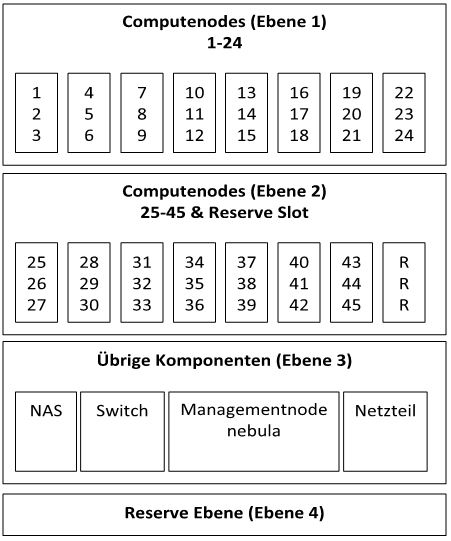
\includegraphics[scale=0.5]{Cluster_Aufbau_Gestell.jpg}
\caption{Physischer Aufbau}
\label{fig:Physischer Aufbau}
\end{figure} 

\textbf{Ebene 1}\newline
24 RPI's sind auf dieser Ebene befestigt worden.

\textbf{Ebene 2}\newline
Es befinden sich 21 RPI's auf dieser Ebene. Es können noch 3 weitere platziert werden.

\textbf{Ebene 3}\newline
Hier wurden alle übrigen Komponenten befestigt. Darunter ist das NAS, der Switch, der Management Node und das Netzteil zu finden.

\textbf{Ebene 4}\newline
Auf dieser Ebene wurde nichts installiert. Sie kann als Reserve Ebene betrachtet werden.

\subsubsection{Kühlung}
Die CPU, RAM und GPU der RPI's wurden mit Aluminium-Kühlkörpern ausgestattet. Die passive Kühlung soll die übertakten CPU's der RPI's am laufen halten.

\subsubsection{Stromversorgung}
\textbf{Compute Nodes}\newline
Die Compute Nodes wurden über die GPIO Pins 2 (5 Volt Anschluss) und 6 (GND Anschluss) über Jumperkabel und weiteren Leiterkabeln, welche zur Verlängerung dienen, mit dem Netzteil verbunden. Es wurde darauf geachtet, dass der Kabeldurchschnitt für eine Anzahl von mindestens 25 Ampere ausreicht, so dass diese nicht durchbrennen.

\textbf{Netzteil}\newline
Am Netzteil wurden Kabelschuhe befestigt, welche es ermöglichen, eine Verbindung mit den Leitern in Richtung RPI's herzustellen. Das Netzteil ist an einer gewöhnlichen Stromschiene angeschlossen.

\textbf{Generelle Verkabelung}\newline
Die Leiter wurden hauptsächlich mit Lüsterklemmen verlängert und auf das zusammenlöten der Komponenten wurde deswegen verzichtet. Dies bietet für neue Verkabelungen eine grössere Flexibilität.

\subsubsection{Kommunikation}
Alle Komponenten, welche eine Netzwekverbindung benötigen, sind über den Switch mit Patchkabeln zusammengeschlossen worden. Es wurde dabei keine spezielle Slotzuweisung des Switches berücksichtigt.


